\section{Relativistic Formulation of Maxwell Theory}

A small comment from last class - we discussed the fact that we could package the energy and momentum into a four vector:
\begin{equation}
    (E, \v{p}) = p^\mu
\end{equation}
and that:
\begin{equation}
    p_\mu p^\mu = p^\mu p^\nu \eta_{\mu\nu} = -(mc)^2
\end{equation}
is a Caismir of the Poincare group/is a Poincare invariant. That is to say - the above is an invariant under boosts/rotations/translations, and has the interpretation that it is the mass of the particle, which is unchanged under all such transformations.

Today, we move onto the relativistic formulation of the Maxwell theory - in your EM courses you have surely seen the 4 Maxwell equations:
\begin{equation}
    \nabla \cdot \v{E} = \frac{\rho}{\e_0}
\end{equation}
\begin{equation}
    \nabla \cdot \v{B} = 0
\end{equation}
\begin{equation}
    \nabla \times \v{B} - \frac{1}{c}\v{E} = \mu_0 \v{J}
\end{equation}
\begin{equation}
    \nabla \times \v{E} + \dot{\v{B}} = 0
\end{equation}
We suspect ahead of time that these are Lorentz invariant (as the wave equation is a consequence of these equations, and it is Lorentz invariant) but there is a way we can write them down such that they are manifestly so.

\subsection{Maxwell under Rotations}
Let's start with rotations, which are a subset of Lorentz transformations. It is not hard to show that the Maxwell equations as written above are already invariant under rotations - let's work this out. The charge density is a scalar, and so:
\begin{equation}
    \rho'(\v{x}') = \rho(\v{x})
\end{equation}
Where $\v{x}' = R\v{x}$, or in index notation, $x^i = R^{ij}x^j$. What of the vector quantities? $\v{E}, \v{B}, \v{J}$ are vector fields, which have a direction at each point in space:

\begin{center}
    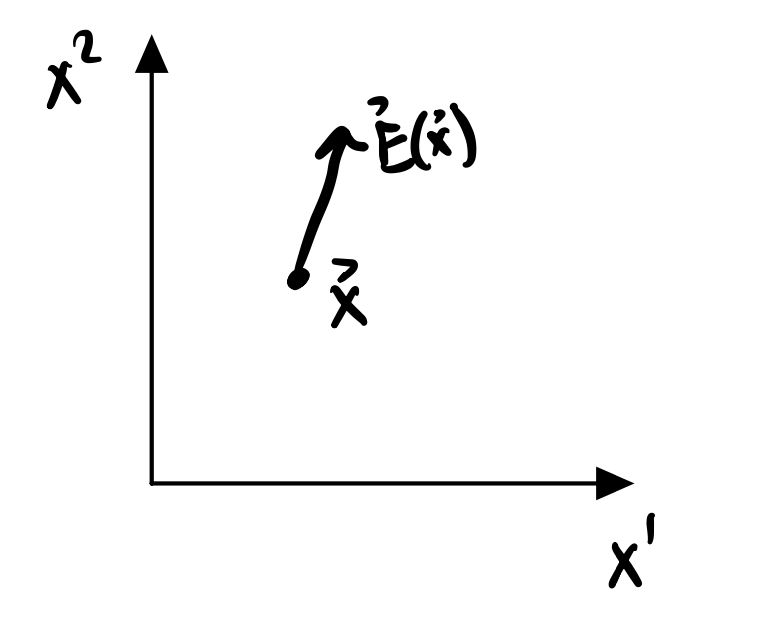
\includegraphics[scale=0.35]{Lectures/Images/lec4-vectorfield.png}
\end{center}

and you can convince yourself that vector fields have the following transformation:
\begin{equation}
    E'_i(\v{x}')dx'^i = E_i(\v{x})dx^i
\end{equation}

\subsection{Gauge Fields}

What we would like to do is generalize this to all Lorentz transformations, where four-vectors $x^\mu = (t, \v{x})$ transform as:
\begin{equation}\label{eq:spacetimecoordLorentztransformation}
    x'^\mu = \Lambda^{\mu}_{\sp\nu}x^\nu.
\end{equation}
The issue now becomes that it is unclear how $\v{E}, \v{B}$ (which are \emph{not} 4-vectors) transform. The main hint is that we may write the electric and magnetic fields in terms of a scalar and vector potential:
\begin{equation}
    \v{E} = -\nabla \phi - \dot{\v{A}}
\end{equation}
\begin{equation}
    \v{B} = \nabla \times\v{A}
\end{equation}
there is a sense in which $\phi, \v{A}$ are more fundamental than $\v{E}, \v{B}$, which we will see later in the lecture.Now, we are back to a problem that we have previously encountered. We have a scalar $\phi$ and a vector $\v{A}$, so it makes sense to package them into a single four-vector, known as the gauge field:
\begin{equation}
    A^\mu = (\frac{\phi}{c}, \v{A})
\end{equation}
The question then becomes whether or not this is a useful definition, and the answer is yes! 

Under Lorentz transformations, we expect:
\begin{equation}
    A_\mu(x')dx'^\mu = A_\nu(x)dx^\nu
\end{equation}
before we move on, it's worth picking apart exactly what this means; if we divide both sides by $dx^\nu$:
\begin{equation}
    A_\mu'(x')\frac{dx'^\mu}{dx^\nu} = A_\nu(x)
\end{equation}

Now, the derivative we can read off from Eq. \eqref{eq:spacetimecoordLorentztransformation}:
\begin{equation}
    \frac{dx'^\mu}{dx^\nu} = \Lambda^{\mu}_{\sp\nu}
\end{equation}
so then:
\begin{equation}
    A_\mu'(x')\Lambda^{\mu}_{\sp\nu}= A_\nu(x)
\end{equation}

\subsection{Field Strength}
Now, we have to check what the implication this is for on the $\v{E}, \v{B}$ - the answer is that we can define the field strength of the gauge field:
\begin{equation}
    F_{\mu\nu} = \p_\mu A_\nu - \p_\nu A_\mu
\end{equation}
where $\p_\mu = \ddpd{}{x^\mu}$. I have a suspicion that $F_{\mu\nu}$ has something to do with $\v{E}, \v{B}$. The first reason is that $F_{\mu\nu}$ is a $4\times 4$ antisymmetric matrix:
\begin{equation}
    F_{\mu\nu} = -F_{\nu\mu}
\end{equation}
which contains 6 independent components, which matches the total number of independent components stored in the $\v{E}, \v{B}$. The other reason is that $F_{\mu\nu}$ is gauge invariant. Last quarter, you noticed that, for an arbitrary scalar function $\chi$, we could transform the scalar/vector potential as:
\begin{equation}
    \phi' = \phi - \p_t \chi, \quad \v{A}' = \v{A} + \nabla \chi
\end{equation}
and under such a transformation $\v{E}, \v{B}$ are invariant. Such transformations are known as gauge transformations, and are labelled by an arbitrary scalar function of spacetime. In order to discuss what happens to $F_{\mu\nu}$ under such transformations, we first act how the gauge field $A_\mu(x)$ transforms under such a transformation:
\begin{equation}
    A_\mu'(x) = A_\mu(x) + \p_\mu \chi
\end{equation}
Let's check this for the 0-th/time component:
\begin{equation}
    A_0' = A_0 + \ddpd{}{x^0}\chi \implies -\frac{\phi'}{c} = -\frac{\phi}{c} + \dpd{}{(ct)}\chi \implies \phi' = \phi - \p_t \chi
\end{equation}
and the story for the spatial components is analogous. With this, let's check how the field strength transforms:
\begin{equation}
    F_{\mu\nu}' = \p_\mu A_\nu' - \p_\nu A_\mu' = \p_\mu(A_\nu + \p_\nu\chi) - \p_\nu(A_\mu + \p_\mu \chi) = F_{\mu\nu} + \p_\mu\p_\nu\chi - \p_\nu\p_\mu\chi = F_{\mu\nu}
\end{equation}
it is invariant! So now we're pretty confident that the components of $F$ will give the components of the $\v{E}/\v{B}$ fields. Let's work them out:
\begin{equation}
    F_{i0} = -F_{0i} = \p_i A_0 - \p_0 A_i = -\frac{1}{c}\p_i \phi - \p_0 A_i = \frac{1}{c}E_i
\end{equation}
\begin{equation}
    F_{12} = -F_{21} = \p_1 A_2 - \p_2 A_1 = \e_{3jk}\p_j A_k = B_3
\end{equation}
(where in the last equality we recall that $B_i = \e_{ijk}\p_j A_k$). Thus for the general component of the B-field:
\begin{equation}
    B_i = \frac{1}{2}\e_{ijk}F_{jk}
\end{equation}
the $\frac{1}{2}$ coming from the fact that when we do the $j, k$ summations we get two nonzero terms. The bottom line of this discussion:
\begin{equation}
    F_{\mu\nu} = \m{0 & -\frac{1}{c}E_1 & -\frac{1}{c}E_2 & -\frac{1}{c}E_3 \\ \frac{1}{c}E_1 & 0 & B_3 & -B_2 \\ \frac{1}{c}E_2 & - B_3& 0 & B_1 \\ \frac{1}{c}E_3 & B_2 & -B_1 & 0}
\end{equation}
why did we do all of this? When we first wrote down the Maxwell equations, we had confusion about how $\v{E}, \v{B}$ transform under Lorentz transformations. Now we have answered it - we can combine $\v{E}, \v{B}$ into $F_{\mu\nu}$ and it is easy to see how this transforms, because we know how $A_\mu$ transforms under Lorentz:
\begin{equation}
    F'^{\mu\nu}(x') = \Lambda^{\mu}_{\sp\lambda}\Lambda^{\nu}_{\sp\rho}F^{\lambda\rho}(x)
\end{equation}
This looks very abstract, but it answers very physical questions. Suppose we have a charged particle, eminating an $\v{E}$-field. I could then get on a bike\footnote{Assuming I was very good at riding a bike and I could go close to the speed of light...} and ask what $\v{E}, \v{B}$-fields I observe - this allows us to answer it.

So far, we have just written down a bunch of definitions we hope would be useful. We had Maxwell's equations, and we wanted to make sure they were invariant under Lorentz transformations. Now, we are in a position to go back to this question, and ask if we can write Maxwell's equations in a way where the Lorentz invariance is manifest.

\subsection{Lorentz Covariant Maxwell Equations}
We require one more definition, that of the dual field strength. We have the field strength:
\begin{equation}
    F_{\mu\nu} = \p_\mu A_\nu - \p_\nu A_\mu
\end{equation}
and then its dual is defined by:
\begin{equation}
    {F^*}^{\alpha\beta} = \tilde{F}^{\alpha\beta} \coloneqq \frac{1}{2}\e^{\alpha\beta\gamma\delta}F_{\gamma\delta}
\end{equation}
where:
\begin{equation}
    \e^{0123} = 1
\end{equation}
and every time two indices are flipped we get a $-1$ sign. The $\frac{1}{2}$ in the definition is there to account for the fact that we get two factors in the summation over $\gamma, \delta$. 

We can explicitly work out the components:
\begin{equation}
    \tilde{F}_{\mu\nu} = \m{0 & B_1 & B_2 & B_3 \\ -B_1 & 0 & \frac{1}{c}E_3 & -\frac{1}{c}E_2 \\ -B_2 & -\frac{1}{c}E_3 & 0 & \frac{1}{c}E_1 \\ -B_3 & \frac{1}{c}E_2 & -\frac{1}{c}E_1 & 0}
\end{equation}
from which we can see that $F, \tilde{F}$ are related via $\v{E} \to c\v{B}, c\v{B} \to -\v{E}$. This is the beginning of a rabbit hole known as electromagnetic duality, and it has lead theorists to believe that there exist magnetic monopoles.

We claim that the dual tensor satisfies:
\begin{equation}
    \p_\mu \tilde{F}^{\mu\nu} = 0
\end{equation}
Let's prove this; fully writing out the dual tensor:
\begin{equation}
    \tilde{F}^{\mu\nu} = \e^{\mu\nu\gamma\delta}(\p_\gamma A_\delta - \p_\delta A_\gamma)
\end{equation}
Now taking the derivative;
\begin{equation}
    \p_\mu \tilde{F}^{\mu\nu} = \e^{\mu\nu\gamma\delta}(\p_\mu\p_\gamma A_\delta - \p_\mu \p_\delta A_\gamma)
\end{equation}
Note that the derivative terms are symmetric under $\mu \leftrightarrow \gamma$ and $\mu \leftrightarrow \delta$, but $\e^{\mu\nu\gamma\delta}$ is antisymmetric under such interchanges; hence the derivative vanishes:
\begin{equation}
    \boxed{\p_\mu \tilde{F}^{\mu\nu} = 0}
\end{equation}
and we call this the \emph{Bianchi identity}. Actually, it is four equations, one for each $\nu = 0, 1, 2, 3$. We can write this identity in terms of electric and magnetic fields:
\begin{equation}
    \nabla \cdot \v{B} = 0
\end{equation}
\begin{equation}
    \nabla \times \v{E} + \dot{\v{B}} = 0
\end{equation}
which we can see are just two of the Maxwell equations - the equations are really Lorentz covariant, because we can write them in terms of $\tilde{F}^{\mu\nu}$, so if they are satisfied in one frame we can easily deduce that they are in a boosted frame.

We then have the other two equations which don't straightforwardsly follow from the Bianchi identity:
\begin{equation}
    \nabla \cdot \v{E} = \frac{\rho}{\e_0}
\end{equation}
\begin{equation}
    \nabla \times \v{B} - \frac{1}{c}\dot{\v{E}} = \mu_0\v{J}
\end{equation}

The charge and current densities satisfy the continuity equation:
\begin{equation}
    \dot{\rho} + \nabla \cdot \v{J} = 0
\end{equation}
at this point, we're Pavlovian dogs who start drooling whenever we see a scalar and a vector together, so we're motivated to define:
\begin{equation}
    J^\mu = (c\rho, \v{J})
\end{equation}
wherein the continuity equation just reads:
\begin{equation}
    \p_\mu J^\mu = 0 
\end{equation}

Under Lorentz transformations:
\begin{equation}
    J'^\mu(x')dx'_\mu = J^\nu(x)dx_\nu
\end{equation}

So let's get back to the remaining two Maxwell equations; you can convince yourself that:
\begin{equation}
    \boxed{\p_\mu F^{\mu\nu} = -\mu_0 J^\nu}
\end{equation}
which is the relativistically covariant form of the Maxwell equations relating the fields to charges/currents.

One thing to point out - when we write this, one thing that is obvious is that if we can write this at all, the current must be conserved. The reason is that if that if I take the derivative $\p_\nu$:
\begin{equation}
    \p_\nu \p_\mu F^{\mu\nu} = -\mu_0 \p_\nu J^\nu
\end{equation}
on the LHS we have a trivial zero (symmetric derivative of an antisymmetric tensor) so:
\begin{equation}
    \p_\nu J^\nu = 0
\end{equation}
the current must be conserved. Said another way, the electromagnetic field can only couple consistently to conserved currents.

A comment - on Tuesday, we discussed the dynamics of free particles. We might ask whether we've solved the problem of charged particles here - the answer is not quite, since throughout we've assumed $\rho, \v{J}$ are smooth and a charged pointlike particle would give rise to a delta-function concentrated charge/current. But we'll see how to deal with this later.

\subsection{Lagrangian Formulation}
We have found the Maxwell equations:
\begin{equation}
    \p_\mu \tilde{F}^{\mu\nu} = 0
\end{equation}
\begin{equation}
    \p_\mu F^{\mu\nu} = -\mu_0 J^\nu
\end{equation}
and we want to know whether we can get these equations from Euler-Lagrange equations that follow from some Lagrangian.

First, we review the situation in point-particle mechanics. Then, we generalize to field theory. Finally, we will specialize to E\& M.

In classical mechanics, we have generalized coordinates $q_i(t)$ for $i = 1, \ldots n$. The action is then:
\begin{equation}
    S = \int dt \mathcal{L}(q_i, \dot{q}_i)
\end{equation}
for $\mathcal{L} = T - U$. The Euler-Lagrange equations are then:
\begin{equation}
    \dod{}{t}\dpd{\LL}{\dot{q}_i} = \dpd{\LL}{q_i}
\end{equation}
and you have solved this, e.g., when $T = \frac{1}{2}\sum_i m_i \dot{q}_i^2$ and $U = U(q_1, \ldots q_n)$. 

We now want to promote these coordinates to fields, $q_i(t) \to \phi_i(t, \v{x})$, and we shall continue with this next lecture.